\documentclass[12pt,a4paper]{article}

% Packages
\usepackage[utf8]{inputenc}    % Unicode support
\usepackage{amsmath,amsfonts}  % Math symbols
\usepackage{graphicx}          % Images
\usepackage{hyperref}          % Hyperlinks
\usepackage{geometry}          % Page layout
\usepackage{caption}           % Captions for figures/tables
\usepackage{cite}              % Citations

% Page layout settings
\geometry{
    top=1in,
    bottom=1in,
    left=1in,
    right=1in
}

% Title information
\title{RoboSurgery}
\author{Matteo Nunziante\thanks{matteo.nunziante@studenti.units.it}}
\date{\today}

\begin{document}

% Title
\maketitle

% Abstract
\begin{abstract}

\end{abstract}

% Keywords
\textbf{Keywords:} keyword1, keyword2, keyword3
\newpage


% Table of contents
\tableofcontents 
\newpage

\section{Abstract}
% Medical applications of Machine Learning are increasingly common.  deformable registration 
% are vast and varied. In image-guided surgery, 
% it allows for precise alignment of preoperative images with the patient's current anatomy, 
% enhancing the surgeon's ability to navigate and operate.

% This Work investigates the applicability of such techniques in the context of rats vats. Because of incomplete knowledge due to unknown organ pose,
%  making planning challenging, we model the problem as a partially observable Markov decision process
%  which allows a general reward based optimization objective and takes uncertainty in temporal evolution and partial observations into account


\newpage
\section{Introduction}
Lung cancer remains a leading cause of cancer-related deaths worldwide, with surgical 
resection offering the best chance for cure in early-stage cases. However, the 
intraoperative environment presents significant challenges, including dynamic 
anatomical changes, limited visibility, and high stakes for patient safety. Assistive 
technologies capable of real-time decision-making and adaptability could greatly 
enhance surgical outcomes. In this context, this thesis explores the potential of 
Partially Observable Markov Decision Processes (POMDPs) and Reinforcement Learning 
(RL) as frameworks for developing intelligent, adaptive, and safe intraoperative 
tools.

% Methodology
\section{Problem Statement}
Over the last decade, 3D models have entered oncologic surgery
as a means to achieve better outcomes in renal and hepatic
surgery [1, 2]. Nevertheless, the integration of 3D models into
the operative field has been lacking due to three main reasons.
Firstly, proper model alignment with the intraoperative anatomy
has proven to be a major challenge due to shifting of organs
during surgery and different patient positioning in surgery ver-
sus during computed tomography [2, 3]. Secondly, automated
organ registra-tion in a continuously moving surgical video
has been another major challenge for many years [4]. Thirdly,
3D model overlay obscures the surgical field, including sharp
surgical instruments which are manipulated, hence creating a
possible hazardous situation rather than facilitating surgery. The
latter occlusion problem has been a longstanding study topic
[5] which, if solved, would further advance various surgical
domains and applications [6]. Already in 2004, Fischer et al. [7]

% Related Work
\section{Related Work}
% Deformable registration refers to the process of aligning multiple three-dimensional 
% images into a common coordinate frame. It quantifies changes in organ shape, size,
% and position, providing a comprehensive understanding of patient anatomy and 
% function. This technique is particularly useful in image-guided surgery and 
% radiotherapy to improve the accuracy of treatments.
\begin{itemize}
    \item Instrument occlusion
    \item DL recognition of anatomical structures
    \item Elastic Regristration
\end{itemize}

While robotic systems have revolutionized minimally invasive surgery, they lack the 
ability to adapt to unexpected intraoperative changes autonomously. POMDPs, with 
their capacity to model uncertainty, and RL, with its learning-based adaptability, 
present a promising synergy for addressing these challenges. However, their 
application to real-time intraoperative decision-making remains unexplored.




% POMDP
% \chapter{Reinforcement Learning}
\section{POMDP}
Formal description of Partially Observable Markov Decision Process as in \cite{Spaan2012}

Formally, a POMDP is a 7-tuple $(S,A,T,R,\Omega,O,\gamma)$, where: \\
$S$ is a set of states, \\
$A$ is a set of actions, \\
$T$ is a set of conditional transition probabilities between states, \\
$R: S\times A \rightarrow \mathbb{R}$  is the reward function. \\
$\Omega$ is a set of observations, \\
$O$ is a set of conditional observation probabilities, \\
$\gamma \in [0,1)$ is the discount factor.


There are at least two causes for the intractability of POMDPs: 1) state space size, and 2) policy size. State-of-the-art POMDP
 methods yield good policies even for POMDP problems with hundreds of thousands of states [7], [8] by trying to limit policy 
 search to state space parts that are reachable and relevant for finding good policies. However, in complex real-world problems
  the state space can be still much larger. In POMDPs with discrete variables, the state space size grows exponentially w.r.t 
  the number of state variables. In order to make POMDPs with large state spaces tractable, there are a few approaches: compressing 
  probability distributions into a lower dimension [12], using factored probability distributions [13], [14], or using particle filtering
   to represent probability distributions [9], [10]. Particle filtering is particularly attractive, because an explicit probability model
    of the problem is not needed. In fact, in order to cope with a complex state space, we use particle filtering in the online POMDP method presented in more detail in Section 3.2.
\section{Variational Bayes}
\section{Reinforcement Learning}
\subsection{PPO}


\newpage
\section{Codebase}
This codebase provides a framework for simulating a surgical robot navigating a deformable gridworld. It includes:
\begin{itemize}
    \item An \texttt{ObservableDeformedGridworld} class for modeling environment states, actions, and transformations.
    \item A C++ module that can be wrapped with pybind11 for Python integration.
    \item Randomized sampling of deformations (stretch and shear) and an obstacle-rich environment.
    \item An infrastructure for step-by-step interaction and reward evaluation, aligning with a POMDP structure.
\end{itemize}
\subsection{State Space}
We are interested in the estimation of the deformaition parameters of an object in a 2D space.
$$s = (\theta)$$

$\theta$ represents the deformation tensor.

\subsection{Action Space}
The action space is the set of all possible actions that the robot can take, 
Forwards, Backwards, Left, Right.
\subsection{Observation Space}
The observation space is the set of all possible observations that the robot can make,
i.e. the presence or absence of an obstacle in its field of view.
\subsection{Bayesian estimation}

rendere il belief indipendente dalla posizione e orientazione del robot, dipenderò unicamente dalla deformazione

$$b(s) = b(theta) * \delta(xyphi = real(xyphi))$$

real(xyphi) = x*
from now on x = xyphi



$$b'_{a,o}(x',\theta') = \eta \cdot \delta(x'=x^*+a) \cdot p(o|x',\theta') \cdot \sum_{x,\theta}p(x',\theta'|x,\theta,a)b(x,\theta)$$
$$ = \eta \cdot \delta(x'=x^*+a) \cdot p(o|x',\theta') \cdot b(x'-a,\theta') $$
$$ = \eta \cdot \delta(x'=x^*+a) \cdot p(o|x',\theta') \cdot \delta (x'-a = x^* )b(\theta') $$
$$ = \eta \cdot \delta(x'=x^*+a) \cdot p(o|x',\theta') \cdot b(\theta') $$
$$ = \eta \cdot \delta(x'=x^*+a) \cdot b'_{a,o}(\theta')$$

dunque a seconda della azione scelta i non zero saranno i 4 x raggiungibili con a

$$p(o|b,a) = \sum_{x,\theta}p(o|x,\theta)b(x.\theta)$$
$$ = \sum_{\theta}p(o|x^*,\theta)b(\theta)$$
% Conclusion
\newpage
\section{Experiments}
\section{Results}




% References
\newpage
\bibliographystyle{plain}
\bibliography{ref}


\end{document}




% \subsection{MDP Solution}
% \subsection{QMDP}

% % \begin{center}
% % 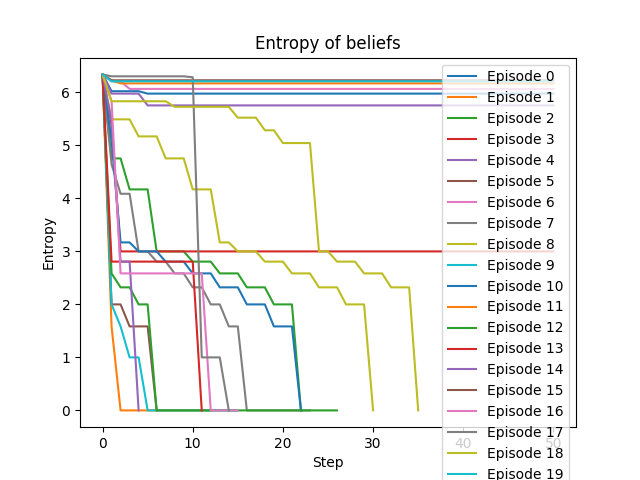
\includegraphics[scale=0.7]{../src/plots/Qentropy_13out20.png}
% % \end{center}

% % reaching target 13 out of 20 times.

% % \subsection{Thompson Sampling}
% % \begin{center}
% %   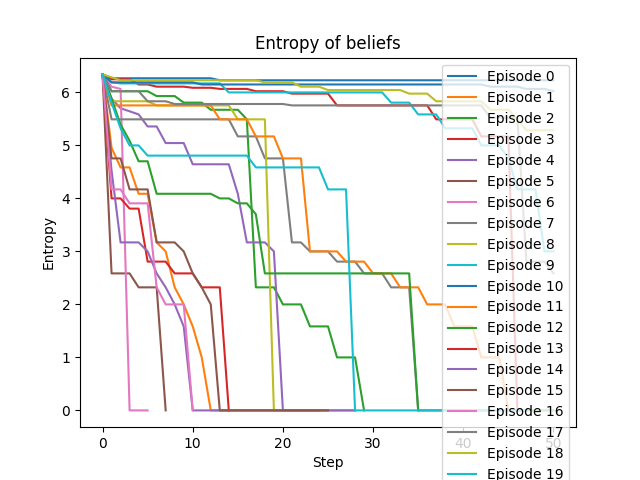
\includegraphics[scale=0.7]{../src/plots/Thompsonentropy_14out20.png}
% % \end{center}
  
% % reaching target 14 out of 20 times.

% % \subsection{Infotaxis}
% % \begin{center}
% %   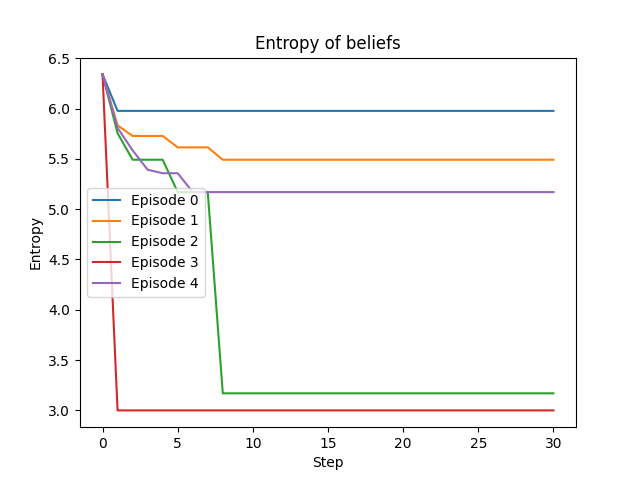
\includegraphics[scale=0.7]{../src/plots/Infotaxisentropy_0out5.png}
% % \end{center}

% % reaching target 15 out of 20 times.

% % \subsection{Information Directed Sampling}
% % \cite{russo2017learningoptimizeinformationdirectedsampling}

% % \begin{center}
% %   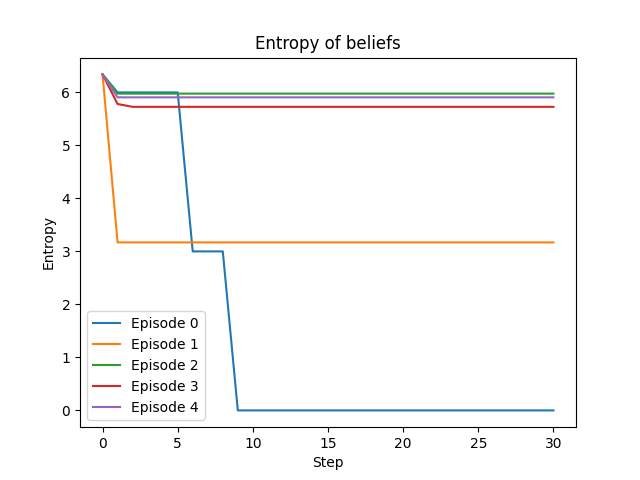
\includegraphics[scale=0.7]{../src/plots/IDSentropy_0out5.png}
% % \end{center}

% reaching target 0 out of 5 times


% \subsection{DQN}


% layout:
% - introduction
% - problem statement
% - related work

% - tecniche 
% - pomdp e variational Bayes

% esperimenti
% discrete continous 

% risultati
% valutazione
% critiche
% prospettive

% materiale aggiuntivo/riassuntivo in appendice \

